%%% Local Variables:
%%% TeX-master: "slides"
%%% End:

\begin{frame}
  
\end{frame}




\begin{frame}
  \begin{center}
    \scalebox{2}{
  \begin{tikzpicture}

    \node<1> at (10mm, 15mm){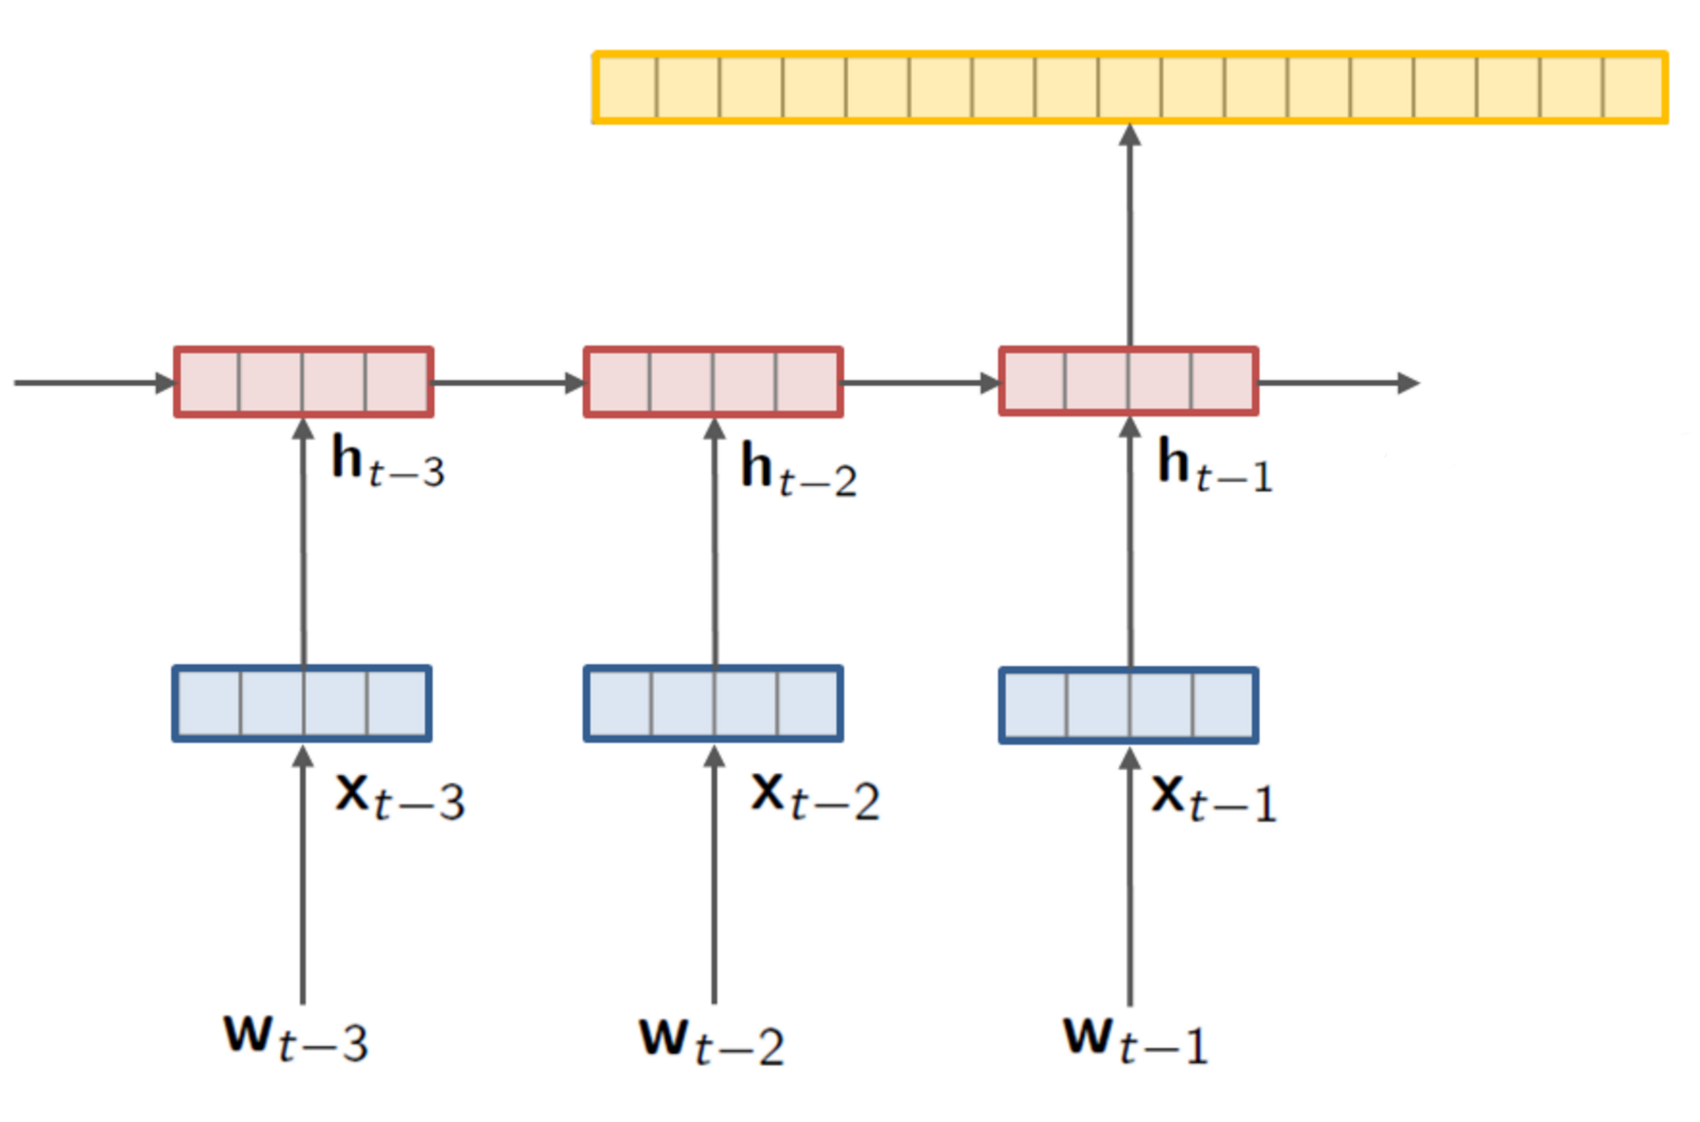
\includegraphics[width=3cm]{rnnlm6}};
    \node[draw,  fill=yellow, thick, rounded corners, scale=0.5] (ana) at (-15mm, 15mm) {Analysis};
    \node[draw,  thick, rounded corners,scale=0.5] (meth) at (0mm, 30mm) {\ Methods\phantom{p}};
    \node[draw,  thick, rounded corners,scale=0.5] (app) at (25mm, 30mm) {Applications};
    \node[draw, thick, rounded corners, scale=0.5] (und) at (35mm, 15mm) {Understanding};
    \node[draw, thick, rounded corners, scale=0.5] (dep) at (25mm, 0mm){Deployment};

    \node[draw, fill=yellow, thick, rounded corners,scale=0.5] (imp) at (0, 0) {Implementation};

    \draw (ana) -- (meth) --(app) -- (und) -- (dep) -- (imp) -- (ana);

  \end{tikzpicture}
}
  \end{center}


\end{frame}

\begin{frame}{Generation Setup (Reminder)}
    \[ \alert<3>{y^*_{1:T}} = \argmax_{y_{\tikzmark{opt}1:T}} \alert<4>{f}(\alert<3>{y_{1:T}}; \tikzmark{input}\alert<2>{x}, \tikzmark{nn}\alert<4>{\theta}) \] 

% \begin{tikzpicture}[
%   remember picture,
%   overlay]

% \node (ptdex) [below left=  of {pic cs:pd}] {Output};
% \node (ptdexa) [below right =  of {pic cs:nn}] {Neural Network};
% \node (ptdexb) [below = of {pic cs:opt}] {Optimization};
% \node (ptdexc) [below = of {pic cs:input}] {Input};
% \draw[->] (ptdex.north) -- ({pic cs:pd}); 
% \draw[->] (ptdexa.north) -- ({pic cs:nn}); 
% \draw[->] (ptdexb.north) -- ({pic cs:opt}); 
% \draw[->] (ptdexc.north) -- ({pic cs:input}); 
% \end{tikzpicture}

  \begin{itemize}

  \item Input \alert<2>{$x_{1:S}$},  \textit{what to talk about}
    \air 

  \item Output text \alert<3>{$y^*_{1:T}$}, \textit{how to say it}
    \air

  \item Model \alert<4>{$f(.; \theta)$}, learned from data
  \end{itemize}
\end{frame}

\begin{frame}{Recurrent Neural Networks}
  \vspace{-0.25cm}

  \begin{center}
    \multiinclude[format=png,start=1,graphics={height=0.85\textheight}]{nmt-noattn}
  \end{center}
\end{frame}


\begin{frame}{RNN Math}
  \textcolor{blue}{Encoder}:
  \[{\mathbf{h}^{x}_s \gets \RNN(\mathbf{h}^{x}_{s-1}, x_s)} \]

  \textcolor{orange}{Context}:
  \[ {\mathbf{c}} = \mathbf{h}^{x}_S \]

  \textcolor{red}{Decoder}:
  \[{\mathbf{h}_t \gets \RNN(\mathbf{h}_{t-1}, y_t)} \]

  Prediction:
  \[ p(y_{t+1}\  |\  y_{1:t}, x) = \softmax( \mathbf{W} [\mathbf{h}_t, \mathbf{c}]) \]

  \pause 

  Generation:
  \[ \argmax_{y_{1:T}} f(y_{1:T}; x, \theta) = \argmax_{y_{1:T}} \log \sum_{t=1}^T p(y_{t}\  |\  y_{1:t-1}, x) \] 

\end{frame}

\begin{frame}{Toy Example: Parenthesis Language}
  \begin{center}
    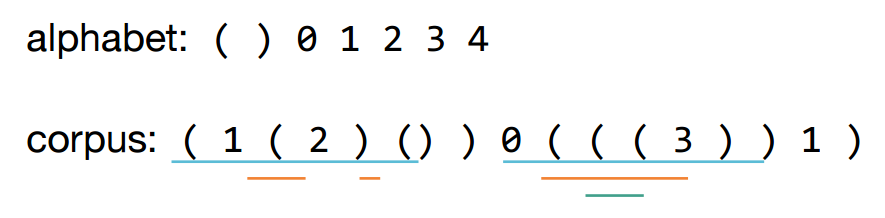
\includegraphics[width=10cm]{parenlang}
  \end{center}
\end{frame}

\begin{frame}{LSTMVis - Parenthesis Language}
  \research{\citet{Strobelt2016} w/ IBM}
  \vspace{-0.25cm}

  \begin{center}
    \movie[width=\textwidth, height=0.85\textheight, poster, showcontrols]{Temporary}{videos/lstmvis1.mp4}
  \end{center}
\end{frame}


\begin{frame}{LSTMVis - Natural Language}
  \research{\citet{Strobelt2016} w/ IBM}
  \vspace{-0.25cm}


  \begin{center}
    \movie[width=\textwidth, height=0.85\textheight, poster, showcontrols]{Temporary}{videos/lstmvis2.mp4}
  \end{center}
\end{frame}


\begin{frame}{Seq2Seq + Attention Model}
  \vspace{-0.25cm}

  \begin{center}
    \multiinclude[format=png,start=1,end=10,graphics={height=0.85\textheight}]{figs/nmt-attn}
  \end{center}
\end{frame}

\begin{frame}{Attention Math}

  \textcolor{blue}{Encoder}:
  \[{\mathbf{h}^{x}_s \gets \RNN(\mathbf{h}^{x}_{s-1}, x_s)} \]


  \textcolor{orange}{Attention}
  \[\alpha \gets  \softmax(   [\mathbf{h}^{x}_1 ; \ldots; \mathbf{h}^{x}_S]^\top \mathbf{h}_{t} ) \ \ \ \ 
  {\mathbf{c}} \gets \sum_{s =1}^S \alpha_s \mathbf{h}_s^{x}  \]

  \textcolor{red}{Decoder}:
  \[{\mathbf{h}_t \gets \RNN(\mathbf{h}_{t-1}, y_t)} \]

  Prediction:
  \[ p(y_{t+1}\  |\  y_{1:t}, x) = \softmax( \mathbf{W} [\mathbf{h}_t; \mathbf{c}]) \]

\end{frame}

\begin{frame}{Seq2SeqVis}
  \research{\citet{strobelt2019s} w/ IBM}
  \vspace{-0.25cm}

  \begin{center}
    \movie[width=\textwidth, height=0.85\textheight, poster, showcontrols]{Temporary}{videos/seq2seq.mp4}
  \end{center}
  
\end{frame}


\begin{frame}
  
  \begin{center}
    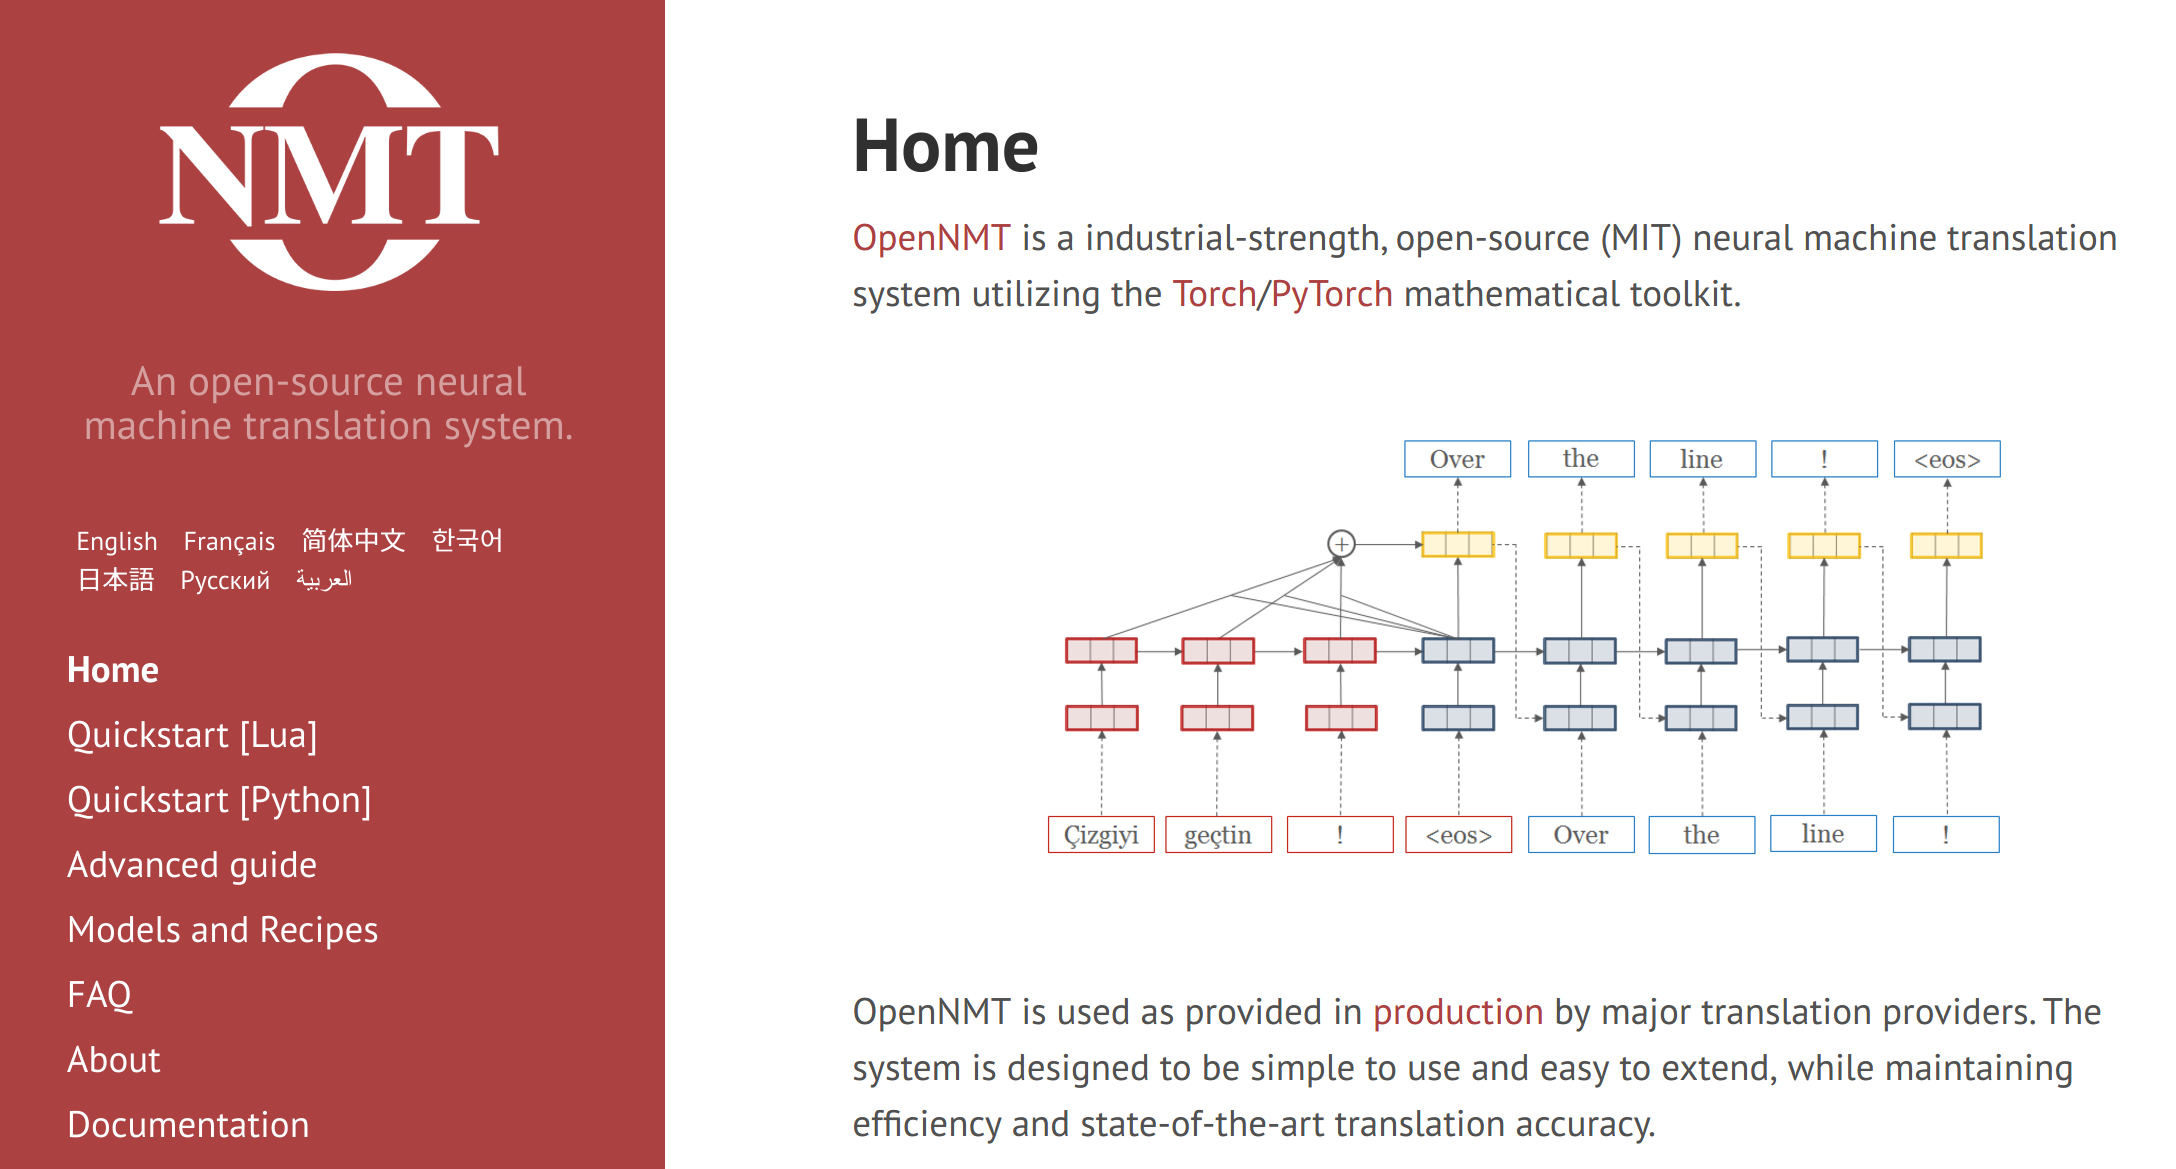
\includegraphics[width=\linewidth]{opennmt}
  \end{center}

\end{frame}

\begin{frame}
  \begin{center}
    
\includegraphics[width=3cm]{OpenNMT}
  \end{center}

  \begin{itemize}
  \item Collaborative open-source project started at Harvard, now self-sustaining.
    \air 
  \item Used in production by Systran, Ubiqus, Booking.com, and others.
    \air
  \item Over 100 developers in France, China, Japan, Portugal, and the US.
    \air
  \item Designed to be research extensible to latest machine translation techniques. 
    \air

  \item Pretrained models for translation as well as everything in this talk.
  \end{itemize}
\end{frame}

\begin{frame}
  \begin{center}
    \hspace*{-9cm}\includegraphics[height=0.5\textheight]{opennmtpanaram.jpg}
  \end{center}
\end{frame}
